\documentclass[main.tex]{subfiles}

\begin{document}

\chapter*{Class 23/08}

\begin{corollary}
	Let~$\mH$ and~$\mB$ be a hypergraphs on the same vertex set. If~${\mB \subseteq b(\mH)^\uparrow}$ and~${b(\mB)^\uparrow \subseteq \mH^\uparrow}$, then~${b(\mH) = \mB^{\min}}$, so~$\mH^{\min}$ and~$\mB^{\min}$ for a blocking pair.
\end{corollary}
\begin{proof}
	We will prove~$b(\mH)^\uparrow = \mB^\uparrow$.

	Let's prove~'$\subseteq$'. We have that~$b(\mB)^\uparrow \subseteq \mH^\uparrow \stackrel{\text{Ex5}}{\implies} b(\mH^\uparrow)^\uparrow \subseteq b(b(\mB)^\uparrow)^\uparrow = b(b(\mB))^\uparrow \stackrel{\text{Thm6}}{=} \mB^\uparrow$.

	Let's prove~'$\supseteq$'. By hypothesis and Exercise~4,~$\mB \subseteq b(\mH)^\uparrow \implies \mB^\uparrow \subseteq (b(\mH)^\uparrow)^\uparrow = b(\mH)^\uparrow$.

	Now,~$b(\mH)^\uparrow = \mB^\uparrow \implies b(\mH) = b(\mH)^{\min} \subseteq \mB^{\min}$.
\end{proof}

\begin{exercise}
	For the hypergraphs~$\mH$ and~$\mB$ below, prova that~$\mH^{\min}$ and~$\mB^{\min}$ form a blocking pair.

	(a) If~$G = (V, E)$ is a graph, take~$$\mH \coloneqq (E, \{E(T) \mid T \text{ is a spanning tree of } G\})$$ and~$$\mB \coloneqq (E, \{\d(S) \mid \emptyset \neq S \subsetneq V\}).$$

	(b) If~$G = (V, E)$ is a graph and~$s, t \in V$ are distinct, take
	$$ \mH \coloneqq (E, \{E(P) \mid P \text { is an~$st$-path in~$G$}\}) $$
	and
	$$ \mB \coloneqq (E, \{\d(S) \mid s \in S \subseteq V \setminus \{t\}\}).$$

	(c) If~$G = (V, E)$ is a graph, take
	$$ \mH \coloneqq (E, \{E(C) \mid C \text { is an odd cycle in~$G$}\}) $$
	and
	$$ \mB \coloneqq (E, \{E \setminus \d(S) \mid \emptyset \neq S \subsetneq V\}).$$
\end{exercise}

A clutter~$\mH$ is binary if~$|F \cap B|$ is odd for all~$(F, B) \in \mE(\mH) \x \mE(b(\mH))$.

\begin{exercise}
	Determine (and prove) which of the clutters in exercise~8 are binary.
\end{exercise}

\begin{exercise}
	Let~$H = (V, \mE)$ be a hypergraph with~$V = [n]$. Suppose~$\mH$ is ``given'' by an oravle that answers queries of the form:
	``Given~$i, j \in V$, is there an edge~$F \in \mE(\mH)$ such that~$i, j \in F$?''. Provide a polynomial-time algorithm (with polynomial number of queries to the oracle) that builds a graph~$G = (V, E)$ such that the packing problem for~$\mH$ is \emph{equal} to the maximum weighted stable set problem for~$G$. (Equality between optimization problems means equal sets and optimization functions)
\end{exercise}

\section*{The Branch-and-Bound Method}
Description of the Branch-and-Bound algorithm:\\
\indent\emph{input.} An MIP formulation~$Ax + Gy \leq b$ and~$x \in \Q^n, h \in \Q^r$. \\
\indent\emph{output.} If the algorithm terminates, it returns an optimal solution for the MIP or answers that no feasible solution exists. \\

\newcommand{\LP}{\mathit{LP}}

The algorithm keeps
\begin{enumerate}[(i)]
	\item a finite list~$L$ of nodes~$N_i$, with~$i \in \N$.
	\item each node~$N_i$ in~$L$ has an associate LP, denoted by~$\mathit{LP}_i$ with optimal value~$z_i$.
	\item a subset~$\xbar{X}$ of at most one feasible solution~$(\xbar{x}, \xbar{y})$ for the MIP with objective value~$\xbar{z}$. If~$\xbar{X} = \emptyset$, we have~$\xbar{z} = -\infty$.
\end{enumerate}

Description: \\
\begin{algorithmic}
	\LineComment{0. Initialize}
	\State $L = \{N_0\}$,~$\LP_0$ is the LP relaxation of~$Ax + Gy \leq b$ with objective function~$c^T x + h^T y$.
	\State $\xbar{X} = \emptyset$,~$\xbar{z} = -\infty$.
	\LineComment{1. Terminate?}
	\If{$L = \emptyset$}
		\If{$\xbar{X} = \emptyset$}
			\State answer ``infeasible''.
		\Else
			\State return the unique element of~$\xbar{X}$.
		\EndIf
	\EndIf
	\LineComment{2. Select Node}
	\State Choose a node~$N_i$ from~$L$.
	\State $L = L \setminus N_i$.
	\LineComment{3. Bound}
	\State Solve~$\LP_i$ (assuming it is bounded)
	\If{$\LP_i$ is infeasible} \Comment{Pruned by infeasibility}
		\State Go to ``1. Terminate?''
	\Else
		Let~$(x^\star, y^\star)$ be an optimal solution for~$\LP_i$ with object value~$z_i$.
	\EndIf
	\LineComment{4. Prune?}
	\If{$z_i \leq \xbar{z}$} \Comment{Pruned by Bound}
		\State Go to ``1. Terminate?''
	\EndIf
	\If{$x^\star \in \Z^n$}
		\State $\xbar{z} = z_i$.
		\State $\xbar{X} = \{(x^\star, y^\star)\}$.
		\State Go to ``1. Terminate?'' \Comment{Pruned by integrality}
	\EndIf
	\LineComment{5. Branch}
	\State Let~$j \in [n]$ such that~$x^\star_j \notin \Z$.
	\State Form two new LPs from~$\LP_i$ by adding the constraints~$x_j \leq \floor{x^\star_j}$ to one and~$x_j \geq \ceil{x^\star_j}$ to the other and add the two corresponding nodes to~$L$.
	\State Go to ``1. Terminate?''
\end{algorithmic}
\vspace{4ex}

\begin{minipage}{0.45\textwidth}
	An example run on
	\begin{optimize}{MIP}
		\text{Maximize } & 55x_1 + 21 x_2 \\
		\text{Subject to } & -x_1 + x_2 \leq 2 \\
		& 8x_1 + 2x_2 \leq 17 \\
		& x \in \Zp^2
	\end{optimize}
\end{minipage}
\begin{minipage}{0.45\textwidth}
	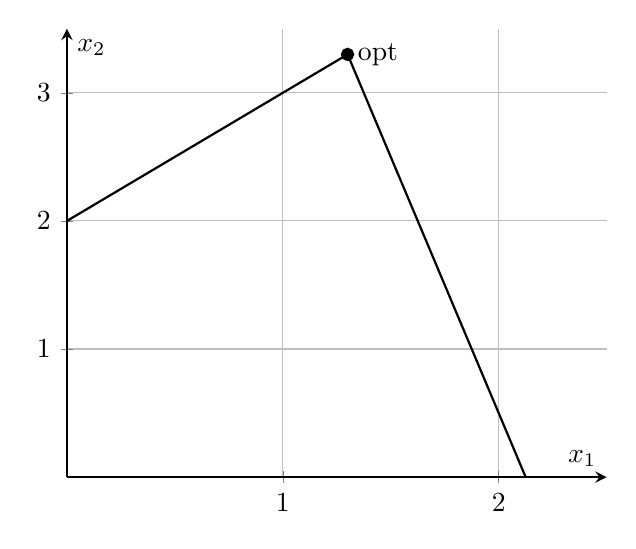
\begin{tikzpicture}
		\begin{axis}[
			xmin=0, xmax=2.5,
			ymin=0, ymax=3.5,
			xtick distance=1,
			axis x line=center,
			axis y line=center,
			grid=both,
			thick,
			xlabel=$x_1$,
			ylabel=$x_2$
		]
			\addplot[domain=0:1.3]{2 + x};
			\addplot[domain=1.3:2.125]{8.5 - 4*x};
			\addplot[mark=*] coordinates {(1.3, 3.3)} node[right]{opt};
		\end{axis}

	\end{tikzpicture}
\end{minipage}

\begin{figure}[h]
	\begin{tikzpicture}[
			ed/.style={->, shorten >=5pt, shorten <=5pt}
		]
		\node[rectangle,inner sep=10pt,draw](A){$x_1 = 1.3$ $x_2 = 3.3$ $z = 140.8$};
		\node[below left = of A,rectangle,draw, inner sep=10pt](B){$x_1 = 1$ $x_2 = 3$ $z = 118$};
		\node[below right = of A,rectangle,draw, inner sep=10pt](C){$x_1 = 2$ $x_2 = 0.5$ $z = 102.5$};
		\node[below left = 2cm and -1cm of C,rectangle,draw, inner sep=10pt](D){$x_1 = 2.125$ $x_2 = 0$ $z = 116.875$};
		\node[below right = 2cm and -2cm of C,rectangle,draw, inner sep=10pt](E){infeasible};

		\draw (A) edge[ed] node[midway,auto]{$x_1 \leq 1$} (B);
		\draw (A) edge[ed] node[midway,auto]{$x_1 \geq 2$} (C);
		\draw (C) edge[ed] node[midway,auto]{$x_2 \leq 0$} (D);
		\draw (C) edge[ed] node[midway,auto]{$x_2 \geq 1$} (E);

		\node[below = .5cm of B]{Pruning by integrality};
		\node[below = .5cm of D]{Pruning by Bound};
		\node[below = .5cm of E]{Pruning by infeasibility};
	\end{tikzpicture}
\end{figure}


\end{document}

